
\cite{bluenoisewronski}

\cite{3288} Ulichney gibt eine Einführung zu \textit{Dithering mit blue noise}. Darunter ist ein abbilden
beliebiger Grauwerte zu einer Menge von blue noise verteilten Schwarz- und Weißwerten zu verstehen.
Somit kann ein für das menschliche Auge gutes Resultat von Grauwerten entstehen, indem nur Schwarz-/
Weißpixel verwendet werden. Denn das menschliche Auge tendiert dazu, benachbarte Pixel verschwimmen
zu lassen und einen Farbwert aus diesen zu generieren. Hat man also einen Grauwert $\textit{p} \in [0,1]$
und will Diesen mit Schwarz-/Weißpixeln approximieren vergleicht man diesen Wert $\textit{p}$ mit den 
Werten aus der Textur und gibt Schwarz (falls \textit{Wert aus der Textur} $\leq$ \textit{p}) oder 
Weiß (falls \textit{Wert aus der Textur} $>$ \textit{p}) aus.


\subsection{Eigenschaften}

Die in \cite{Pet17} vorgestellten blue noise Texturen und ihre Eigenschaften geben 
Aufschluss über ihre Wirksamkeit. Deshalb werden im Folgenden, die dort bereit 
gestellten Texturen verwendet, welche anhand des in \cite{ulichney1993void} 
vorgestellten Algorithmus erstellt wurden.
Die korrespondierenden Spektren wurden mit Hilfe von \cite{FFTProgWeb} erstellt.

\subsubsection{Uniformität}
Wie bereits erwähnt, entsteht der neue Grauwert anhand einer Mittlung über 
mehrere benachbarte Pixel. Aufgrund dessen muss für die Wahrscheinlichkeitsfunktion, dass
ein schwarzer Pixel bei der Generierung ausgeben wird  ($\textit{p} \in [0,1]$) gelten: 

\begin{equation}\label{eq:uniformitaet}
    P(n \leq p) = p
\end{equation}

Die Uniformität(lat. \textit{uniformitas}-Einförmigkeit) garantiert uns dieses
Verhalten $\forall p \in [0,1]$. Die zugehörige konstante Wahrscheinlichkeitsdichte
lässt sich einfach zur Echtzeit umsetzen mit Hilfe von (pseudo-)zufälligen Zahlen.

Mit der in \cite{WhiteNoiseGenerator} erstellten white noise Textur,
\begin{figure}[H]\label{pic:whitenoiseFFT}
    \centering
    \begin{minipage}[t]{0.45\linewidth}
        \centering
        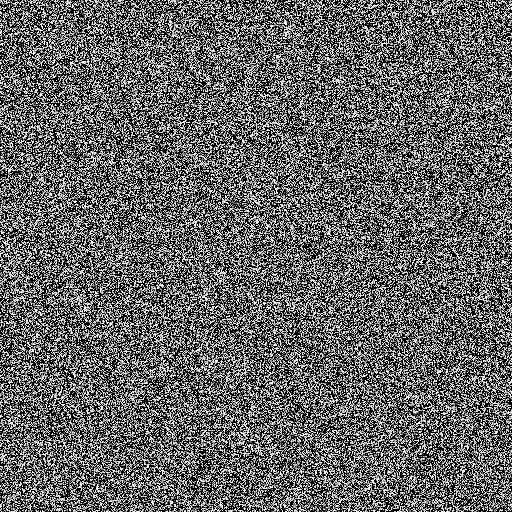
\includegraphics[width=\linewidth]{content/BlueNoise/Bilder/whitenoise.png}
        \caption{$512^{2}$ white noise Textur}
    \end{minipage}
    \hfill
    \begin{minipage}[t]{0.45\linewidth}
        \centering
        
\includegraphics[width=\linewidth]{content/BlueNoise/Bilder/FFT_whitenoise.png}
        \caption{Amplitudenspektrum $512^{2}$ white noise Textur}
    \end{minipage}
\end{figure}

ergibt sich eine typische Amplitudendichte. Zufällig verteilt, über alle 
Frequenzen hinweg. Die folgende Rotationssymmetrie lässt sich \cite{kiencke2009signale}
erklären, da wir die Dimension der Phase des Signals nicht betrachten.
Allerdings lassen sich noch deutlich
ähnlichfarbende Pixelverbünde erkennen.i.e niedere Frequenzen in der
Frequenzdomäne erkennen.

\subsubsection{Isotropie}

Die Isotropie(altgr. \textit{isos}-gleich und \textit{tropos}-Richtung)
einer blue noise Textur wird ausgenutzt. Dabei haben wir in allen
Dimensionen (in dieser Arbeit werden Texturen mit zwei benutzt) 
die Unabhängigkeit einer Eigenschaft. Um uns dies an einem Gegenbeispiel 
klar zu machen, schauen wir uns das Bayer-Pattern, sowie seine korrespondierende
Amplitudendichte an.

\begin{figure}[H]\label{pic:bayerPatternFFT}
    \centering
    \begin{minipage}[t]{0.45\linewidth}
        \centering
        
\includegraphics[width=\linewidth]{content/BlueNoise/Bilder/BayerMatrix.png}
        \caption{$512^{2}$ bayer pattern Textur}
    \end{minipage}
    \hfill
    \begin{minipage}[t]{0.45\linewidth}
        \centering
        
\includegraphics[width=\linewidth]{content/BlueNoise/Bilder/FFT_BayerMatrix.png}
        \caption{Amplitudendichte $512^{2}$ bayer pattern Textur}
    \end{minipage}
\end{figure}

In der Frequenzdomäne ist zu erkennen, das die Amplitudendichte in einzelnen
Punkten organisiert ist. Diese lassen sich durch die vorhandenen
Richtungen der Textur erklären. Speziell in zwei Richtungen ist eine sich
wiederholende Pixelsequenz zu erkennen.
Allerdings wollen wir in alle Richtungen eine gleiche(Isotropie!) 
Verteilung. Durch dieses Bayer Pattern entstehen unbefriedigende 
Artefakte in Echtzeitanwendungen, so in (aktuellen) Spielen 
\cite{bluenoisewronski} zu sehen. Bieten allerdings eine sehr effiziente
Verwendung, da sehr leistungssparende GPU Befehle.

\subsubsection{Niedrige Frequenzen}

Niedrige Frequenzen sind in einer blue noise sehr wenig bis gar nicht 
vertreten. Dies ist an dem schwarzen Ring innerhalb der Amplitudendichte
zu erkennen\ref{pic:blueNoiseFFT}. Oder in der Zeitdomäne, an dem 
Abhandensein von gleichfarbigen Pixelbündeln. Genau dies wollten wir 
erreichen.
Außerdem haben wir aus den vorherigen Beispielen gesehen: Wir wollen 
eine Uniformität \ref{eq:uniformitaet} und eine gleichmäßige Verteilung
in allen Richtungen.

\begin{figure}[H]\label{pic:blueNoiseFFT}
    \centering
    \begin{minipage}[t]{0.45\linewidth}
        \centering
        
\includegraphics[width=\linewidth]{content/BlueNoise/Bilder/LDR_LLL1_0.png}
        \caption{$512^{2}$ blue noise Textur}
    \end{minipage}
    \hfill
    \begin{minipage}[t]{0.45\linewidth}
        \centering
        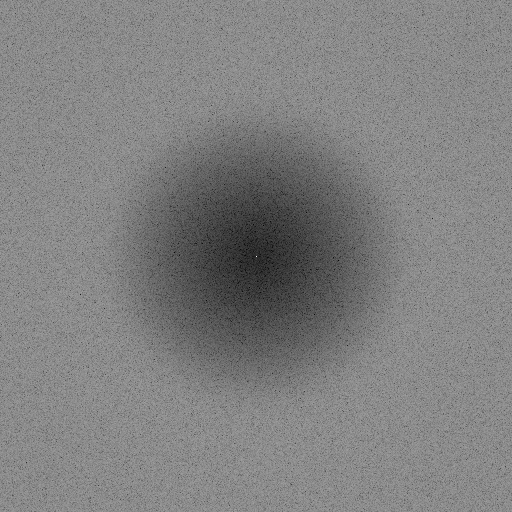
\includegraphics[width=\linewidth]{content/BlueNoise/Bilder/FFT_LDR_LLL1_0.png}
        \caption{Fourier Spektrum $512^{2}$ blue noise Textur}
    \end{minipage}
\end{figure}

Wie in der Abbildung zu sehen ist, haben wir hier die erwünschte
Rotationssymmetrie(Isotropie). Außerdem ist die Uniformität wie 
bei der white noise (bloß ausschließlich bei höheren Frequenzen)
zu erkennen. 

\subsubsection{Kachelung}
Bayer Pattern sowie auch white noise lassen sich einfach zur Echtzeit berechnen. Bei blue noise texturen 
sieht das hingegen anders aus. Für diese Art von Textur müssen wir vor Start der Anwendung eine
Vorberechnung machen. Daher stellt sich nun die Frage, wie groß (welche Auflösung) die Textur haben sollte. 
Aufgrund des Aufbaus von aktueller Grafikhardware \cite{turingarchitecture} wollen wir diese Textur
soweit oben wie möglich in der Cachehierarchie halten.(L1 96KByte, L2 6MByte).
\begin{figure}[H]\label{pic:tiledBlueNoiseFFT}
    \centering
    \begin{minipage}[t]{0.45\linewidth}
        \centering
        
\includegraphics[width=\linewidth]{content/BlueNoise/Bilder/BlueNoise64Tiled.png}
        \caption{$512^{2}$ bayer pattern Textur}
    \end{minipage}
    \hfill
    \begin{minipage}[t]{0.45\linewidth}
        \centering
        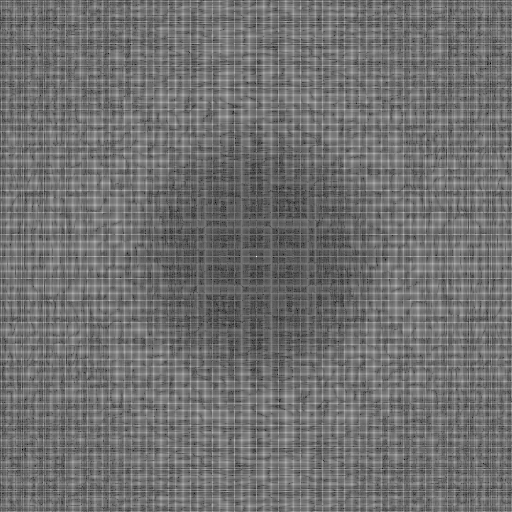
\includegraphics[width=\linewidth]{content/BlueNoise/Bilder/FFT_BlueNoise64Tiled.png}
        \caption{Fourier Spektrum $512^{2}$ bayer pattern Textur}
    \end{minipage}
\end{figure}

In \ref{pic:tiledBlueNoiseFFT} lässt sich der blue noise Charakter wieder anhand des
wenigen niederen Frequenzanteils erkennen. Wiederholungen sind in der Zeitdomäne schwerer zu erkennen,
wohingegen man bereits bekannten Effekt von Bayer Pattern im Frequenzbereich \ref{pic:bayerPatternFFT}, also Wiederholungen,
erkennen kann. Jedoch weniger deutlich, weshalb man diese Kacheln als eine gute Approximation für eine
entsprechend größere Textur halten kann. Vorallem in Anbetracht der bereits angesprochenen 
Performancevorteile.
